\documentclass[10pt]{article}
\usepackage{hyperref}
\usepackage[utf8]{inputenc}
\usepackage{graphicx}
\usepackage{tikz-cd}
%\title{Report for Automatic Program Analysis project 1}
\title{Automatic Lua Code Analysis}
\author{Eduard van der Bent \and Frank Dedden \and Wilco Kusee \and Falco Peijnenburg}

\begin{document}
\maketitle

% Omschrijving van de code
% - Architectuur DONE
% - Howto compile DONE
% - Howto run
% - Dependencies DONE
% - Design choices / highlevel description

\section{Introduction}

For this assignment we have used monotone frameworks to eliminate dead code inside Lua.

\section{Architecture} %herschrijven
% TODO: komen er nog meer bestanden?
When we take a look inside the \texttt{analysis/src} directory, we can see the following files and directories:
\begin{itemize}
	\item \texttt{GLua/}
	\item \texttt{GLuanalysis/}
	\item \texttt{Graphviz.hs}
	\item \texttt{LiveVariables.hs}
	\item \texttt{Main.hs}
	\item \texttt{MonotoneFramework.hs}
	\item \texttt{Reachable.hs}
	\item \texttt{SignAnalysis.hs}
\end{itemize}

Inside the \texttt{GLua} directory, we can find our implementation of a Lua parser. This parser is implemented in the Attribute Grammer system using the \texttt{uuagc} compiler. It creates an abstract syntax tree of the Lua language. % Leggen we niet verder uit, is niet echt onderdeel van het practicum

The \texttt{GLuanalysis} directory houses the Attribute Grammar system that is used for the analysis of the Lua code. \texttt{AG/ControlFLow.ag} is the AG code that creates a control flow graph from the abstract syntax tree. This graph is later used to construct a monotone framework in the file \texttt{MonotoneFramework.hs}. This monotone framework is then used for analysing the input code.\\
There are three instances of the monotone framework: live variable analysis, sign analysis and reachability analysis.
\texttt{LiveVariables.hs} provides functions that check wether the variables in the input Lua code are either dead or alive.\\

Similarly \texttt{reachable.hs} and \texttt{SignAnalysis.hs} check the code for reachable expressions and perform the sign analysis.\\
\texttt{Main.hs} provides some easy to use functions for applying the analyses that are found in the files described above.

\section{Compiling the code}
% TODO: de mainfile wordt misschien nog aangepast? dus het runnen ook?

Compiling and running the code is quite easy. However you have to be sure that all the dependencies are installed beforehand. One of those dependencies (the GLua parser) is included in the project by default. This is because of issues related to UUAGC.

GLuanalysis can be installed as follows. 
\begin{lstlisting}[frame=single,numbers=none,caption=Compiling the project]
cd analysis && cabal configure && cabal build
\end{lstlisting}

This runs both the uuagc compiler and the GHC compiler, creating a executable called \texttt{gluanalysis} in the \texttt{analysis/dist/build/gluanalysis} directory.

\section{Running the analyser}
The analyser takes code input from stdin and writes its results to stdout. Running the analyser with an example file is done as follows:

\begin{lstlisting}[frame=single,numbers=none,caption=Running with an example file]
cat  examples/example1.lua | dist/build/gluanalysis/gluanalysis
\end{lstlisting}

This assumes the current working directory is set to \texttt{analysis/}.

\section{Lattices and Analysis}
Our analysis consists of finding dead code. To accomplish this we use three forms of analysis. The first one is a "reach" analysis, where we check if every node in the control flow graph of the program can be reached from the starting node. Nodes that are unreachable, are dead code.
The second analysis that is done, is Live Variable analysis. This is done to check for superfluous assignments. Nodes that have an assignment in them, but that value is not present in the exit label of that node, are dead code.
The final analysis is Sign Analysis. This is done to check conditionals to check for liveness in their branches. Every node that does not have sign information at the end of the analysis is dead code.
The result of these analyses is combined, checking for every node if it is dead in one of the analysis. If it is dead in at least one analysis, it is considered dead code.\\

The lattices are defined as follows: \\ 
Reach Analysis: \\
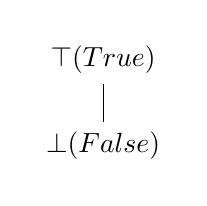
\begin{tikzpicture}
\matrix (a) [matrix of math nodes, column sep=0.6cm, row sep=0.5cm]{
\top (True)\\
\bot (False)\\};
\draw (a-1-1) -- (a-2-1);
\end{tikzpicture}

Live Variables Analysis: \\

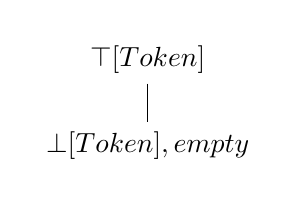
\begin{tikzpicture}
\matrix (a) [matrix of math nodes, column sep=0.6cm, row sep=0.5cm]{
\top [Token] \\
\bot [Token],empty \\};
\draw (a-1-1) -- (a-2-1);
\end{tikzpicture}

Sign Analysis: \\

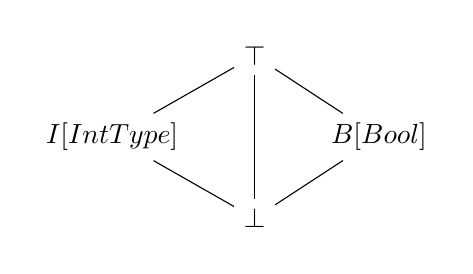
\begin{tikzpicture}
\matrix (a) [matrix of math nodes, column sep=0.6cm, row sep=0.5cm]{
& \top \\
I [IntType] & & B [Bool] \\
& \bot \\};
\draw (a-1-2) -- (a-2-1);
\draw (a-1-2) -- (a-2-3);
\draw (a-1-2) -- (a-3-2);
\draw (a-2-1) -- (a-3-2);
\draw (a-2-3) -- (a-3-2);
\end{tikzpicture}\\
IntType is either Positive, Negative or Zero.\\

For the "reach" and Live Variable analysis, join is defined as the union. For Sign Analysis, we merge existing information of all the signs with the new information from the assignments in the nodes. As far as we know, we do not make use of widening.

\section{Limitations}
We did not manage to properly make the embellished part of the monotone framework work, therefore in all analyses there is mild / severe poisoning when trying to analyze programs with functions.

We can not handle the following lua constructs: local declarations and functions, for loops, tables and anonymous functions.

We can handle the following lua constructs: Definitions, Function calls, Labels and Goto's, Breaks, Continues, Do-blocks, While, Repeat and If.


\section{Example}
<<<<<<< HEAD
In this section we will explain a running example. The code used for the example is the following:\\

x = 1\\
b = function(f)\\
if f then\\
a = f\\
else \\
a = f\\
end\\
return a\\
end\\
x = b(true)\\
y = x\\
if not x then\\
print(y)\\
end\\
x = true\\
while not x then\\
print(y)\\
end\\

Its associated control flow graph is:

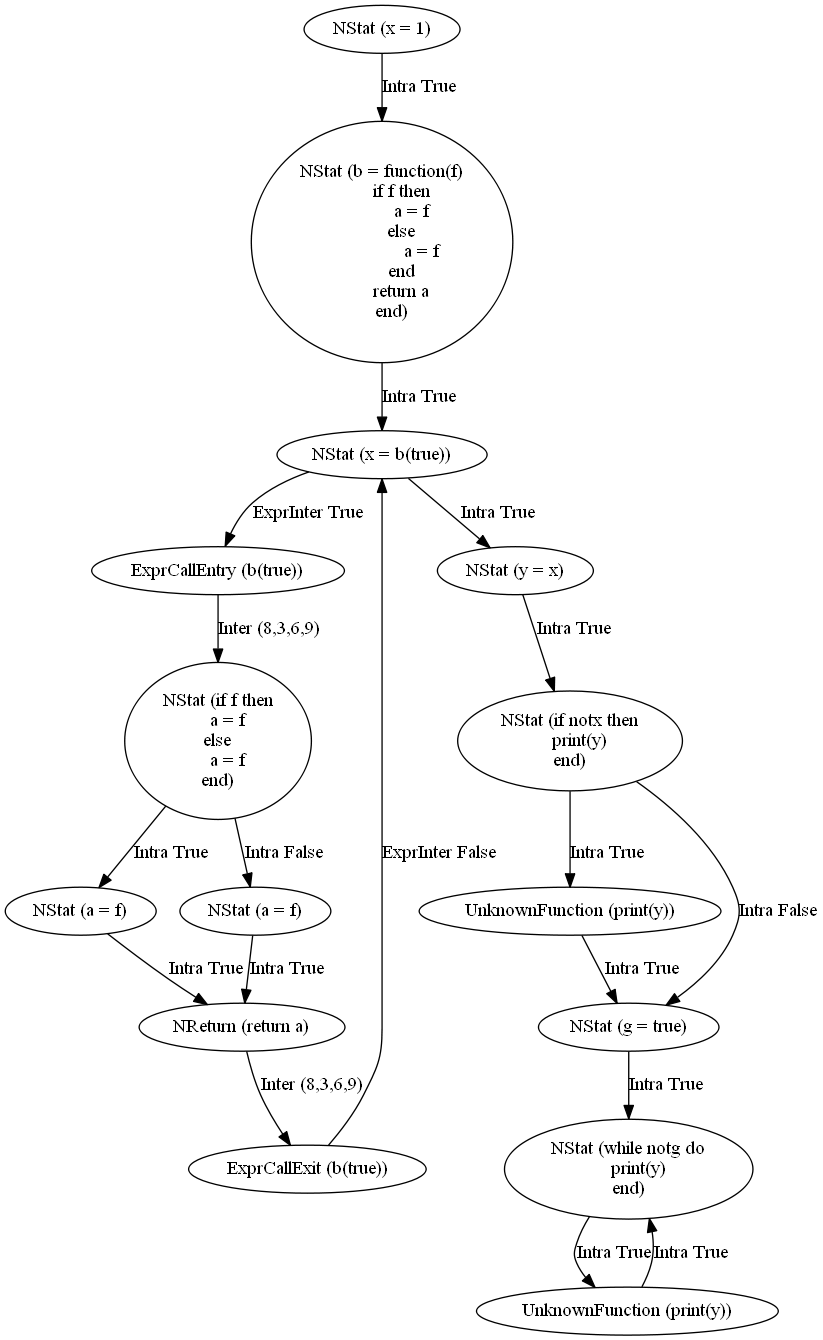
\includegraphics[scale=0.45]{utTesta.png}

=======
In this section we will explain a running example. The code used for the example is the following, and its associated control flow graph can be seen in figure \ref{fig:cfg}.\\

\newpage
\begin{lstlisting}[frame=single,numbers=left,caption=Simple example] % lstlisting kent geen Lua, dus maar geen syntax highlighting
x = 1
b = function(f)
    if f then
        a = f
    else
        a = f
    end
    return a
end

x = b(true)
y = x

if not x then
    print(y)
end

x = true
while not x then
    print(y)
end
\end{lstlisting}
\begin{figure}[htp]
    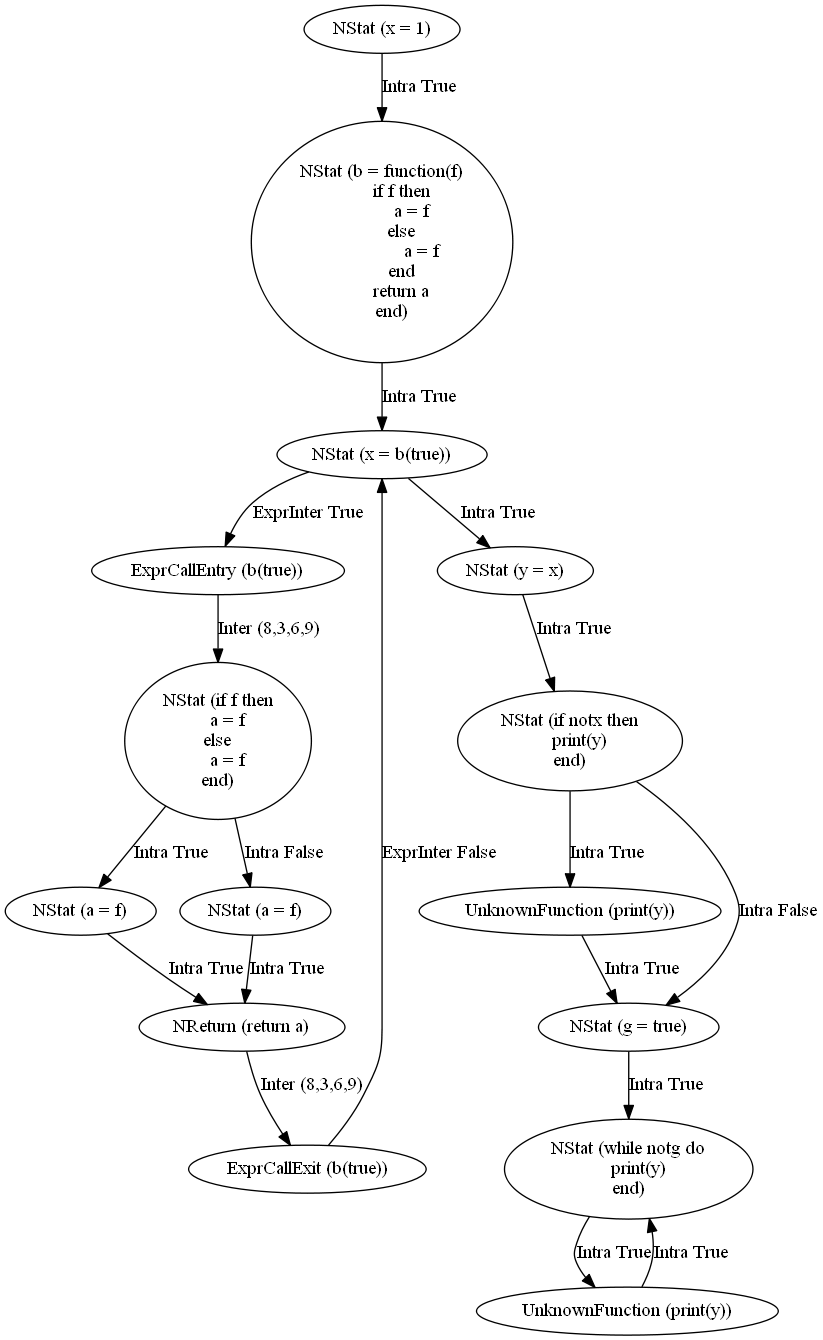
\includegraphics[scale=0.45]{utTesta.png}
    \caption{Control flow graph of the example}
    \label{fig:cfg}
\end{figure}
>>>>>>> 1cfa6e455267048e7420d24c8a3aefda7349ba0c
First of all we discuss the reach analysis. The first node is always reachable, and since there are no nodes without a parent, everything is reachable in this case.\\
Second of all is the Live Variables analysis. The first assignment of x is done but it is not used when x gets its next assignment, so it is dead code.\\
Finally, the Sign Analysis is done. When g is assigned true, the condition of the while loop will never be true. This means that the while-block is dead, and we choose not to visit the nodes of this block in the analysis. This means that the nodes of the block will have bottom as their value, and it is marked as dead code.\\
More interesting is that we do not mark the if-block as dead code. When calling a top-level function, which can also be called from outside the program, we cannot safely make assumptions about the signs of the arguments - we could then incorrectly mark parts of the function as dead code. We thus have to assume that all arguments of a function have Top as their signs. This means that in the program x will have Top as its sign.

\end{document}
